%%%%%%%%%%%%%%%%%%%%%%%%%%%%%%%% 
\section{The Cold Electronics (CE)} 
\label{sec:detectors-fd-ref-ce}

The TPC read-out electronics are referred to as the ``Cold Electronics'' (CE) because they will reside in LAr,
mounted directly on the APA front-end (Figure~\ref{fig:elec_CMBonAPA}).
This will minimize channel capacitance and noise by keeping the length of the connection between an anode wire
and its corresponding electronics input to an absolute minimum.
The CE will be implemented as ASIC chips using CMOS technology,
which performs well at cryogenic temperatures,
and will provide amplification, shaping, digitization, buffering and multiplexing (Mux) of the signals.
The scope of the CE subsystem includes the design, procurement, fabrication, testing,
delivery and installation of the CE, the components of which are:
\begin{itemize}
\item Front-end electronics cards installed on the APAs;
\item Signal feedthroughs;
\item Power supplies and cabling.
\end{itemize}
The most significant requirements for the CE are to:
\begin{itemize}	
\item Read out the TPCs and transmit their data to DAQ;
\item Operate for the life of the facility without significant loss of function;
\item Record the channel waveforms continuously without dead time;
\item Use only materials that are compatible with high-purity liquid argon;
\item Provide sufficient precision and range in the digitization to satisfy the KPP.
\end{itemize}

The CE architecture is manifested in the Cold Mother Board assembly (CMB),
which consists of an analog mother board with a digital ASIC mezzanine (Figure~\ref{fig:elect_schem}).
Each APA is instrumented with 20 CMBs, for a total of 2,560 channels per APA.

The analog mother board is instrumented as a 128-channel board which uses eight 16-channel FE ASICs,
eight 16-channel ADC ASICs, low-voltage regulators, and input-signal protection.
The 16-channel FE ASIC provides amplification and pulse shaping.
The 16-channel ADC ASIC comprises a 12-bit digitizer, local buffering,
and an 8:1 Mux stage with two pairs of serial readout lines in parallel.
This has already been prototyped and tested,
using a commercial FPGA to perform the role of the digital ASIC (Figure~\ref{fig:elec_CMBpix}).

The Cold Digital Data (COLDATA) ASIC and its voltage regulators are mounted on the digital ASIC mezzanine.
The COLDATA ASIC provides:
\begin{itemize}
\item The communication protocol with the data acquisition system (DAQ)
\item The control required to program and read out the FE and ADC ASICs
\item The system clock interface
\item Four 4:1 Muxs that combine 16 serial lines from the ADCs of eight channels each into four serial lines of 32 channels each
\item Four 1-Gbps serial drivers that form the data link to DAQ
\end{itemize}
The data rates will not be high enough to require the use of optical fibers in the cold,
nor is there a need for zero suppression or data compression.
This greatly reduces the complexity of the COLDATA ASIC, with a corresponding decrease in overall risk,
including risk of failure-to-implement (within a fixed schedule and budget)
and risk of device failure during long-term operation.
Data will be driven to DAQ through copper cable utilizing low-voltage differential signaling (LVDS).
Output data cables will go to a signal feedthrough and from there to an external crate mounted nearby.
Under DAQ scope, further data processing is done in the external crate
and data is transmitted via optical fiber to front-end computers.

\begin{cdrfigure}[The front end electronics as mounted on an APA]{elec_CMBonAPA}{The front end electronics,
shown in the red circle, as mounted on an APA.}
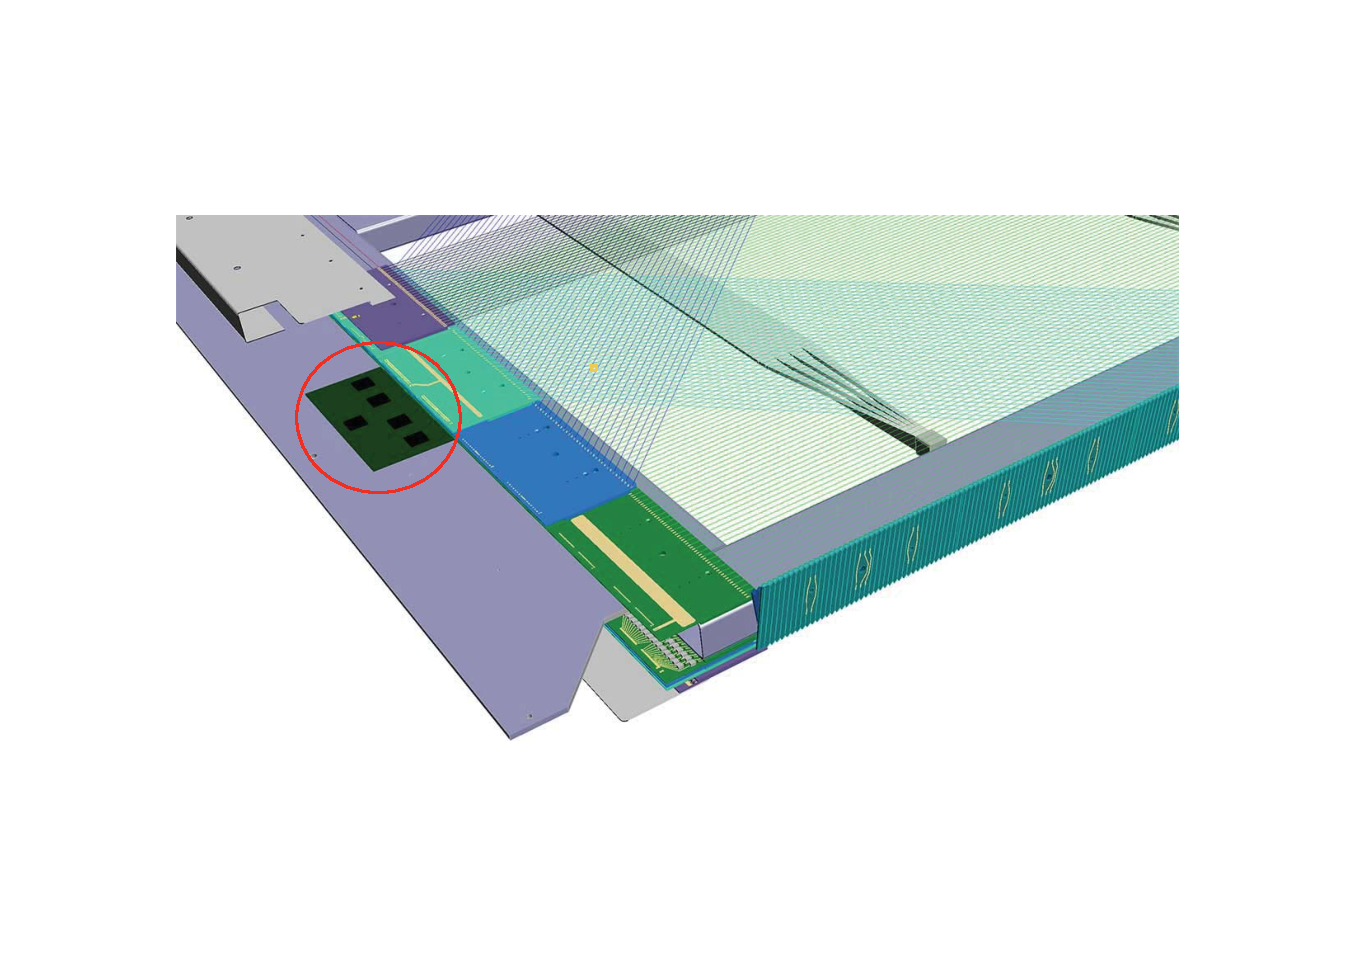
\includegraphics[width=1.00\linewidth]{elec_CMBonAPA_1.pdf}
\end{cdrfigure}
\begin{cdrfigure}[The CE Architecture]{elect_schem}{The CE Architecture. The basic unit is the 128-channel CMB}
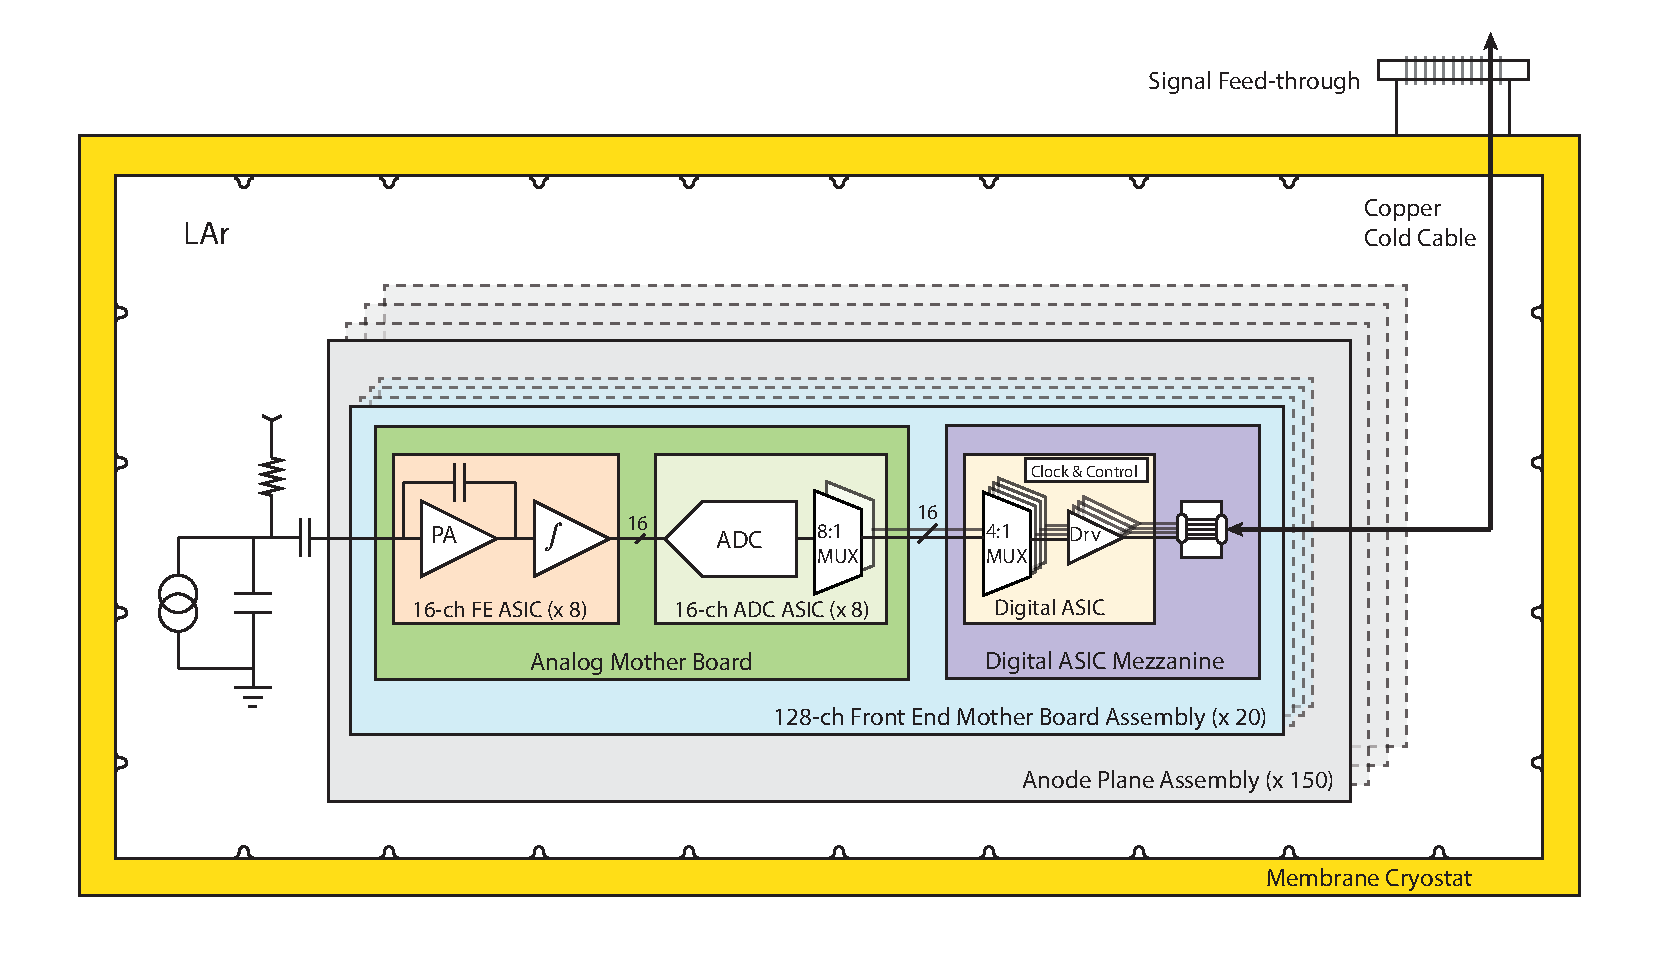
\includegraphics[width=\linewidth]{elect_schem.pdf}
\end{cdrfigure}
\begin{cdrfigure}[Functional Block Diagram of the Cold Digital Data (COLDATA) ASIC]{elec_COLDATAfig}{Functional Block Diagram of the Cold Digital Data (COLDATA) ASIC}
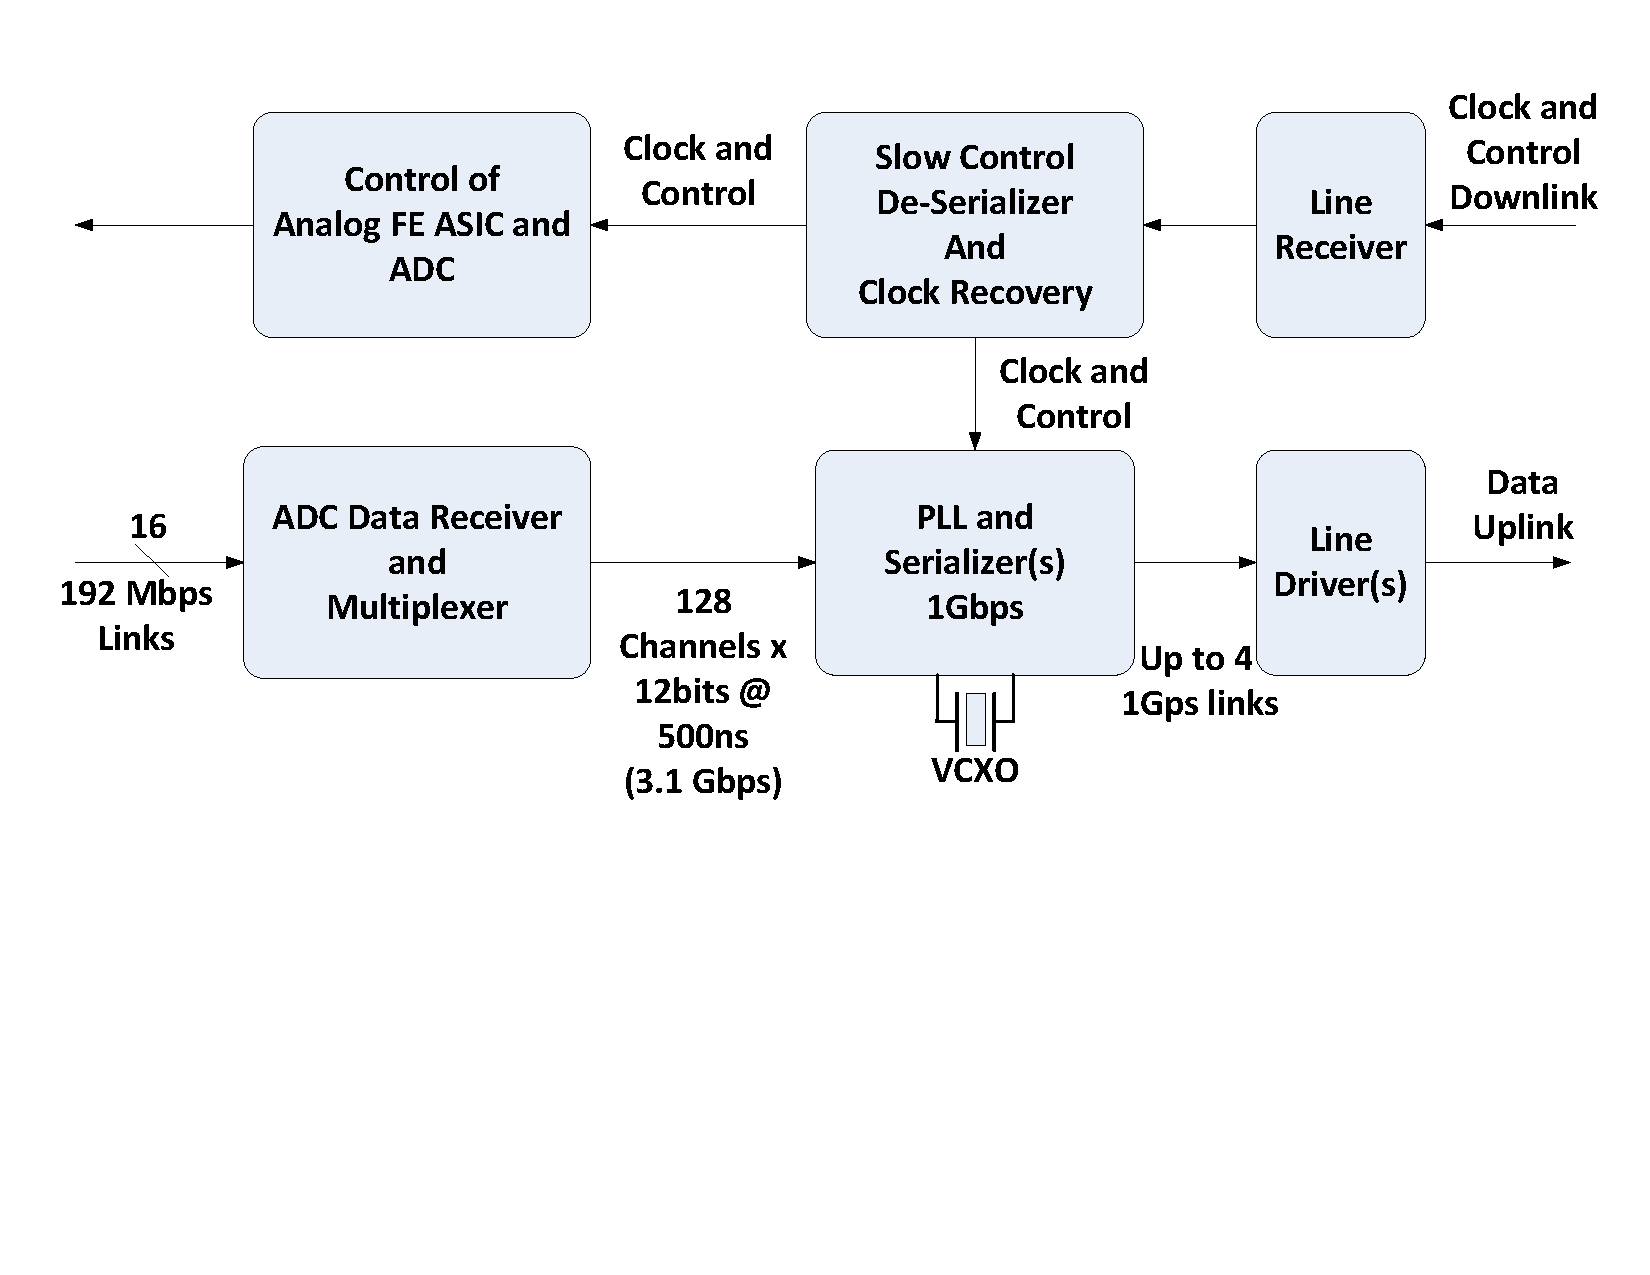
\includegraphics[width=6in]{elec_COLDATAfig.pdf}
\end{cdrfigure}


Here is a sample table:

\begin{cdrtable}[short]{cc}{label}{long}  %The third argument (reads {cc}) can use c, l, r or p{some length} 
% but please do not include lines like “|c|l|l|”. It CAN look like {cll} or {llp{3cm}}, for instance.
Header Column1 & Header Column 2 \\ \toprowrule
Row 1 & First \\ \colhline
Row 2 & Second \\ \colhline
Row 3 & Third \\
\end{cdrtable}
